\documentclass{beamer}
\setbeamercovered{invisible}
\usepackage{listings}
\usepackage{textcomp, fontenc, inputenc}
\renewcommand{\ttdefault}{pcr}

%\AtBeginSection{\frame{\sectionpage\tableofcontents[currentsection]}}
%\AtBeginSubsection{\frame{\subsectionpage\tableofcontents[currentsubsection]}}

\usecolortheme{albatross}
\usebackgroundtemplate%
{%
  
\includegraphics[width=\paperwidth,height=\paperheight]{box.jpg}%
}

\lstset{
  language=Scala,
  showlines=true,
  basicstyle=\scriptsize\ttfamily\color{black},
  rulesepcolor=\color{black},
  backgroundcolor=\color{yellow!10},
  identifierstyle=\color{black},
  keywordstyle=\bfseries\color{blue},
  stringstyle=\color{teal},
  commentstyle=\itshape\color{red},
  showstringspaces=false,
  numbers=left,
  firstnumber=1,
  numberstyle=\color{white},
  columns=fixed,
  keepspaces=true,
  frame=tlb,
  tabsize=2,
  extendedchars=true,
  resetmargins=true,
  breaklines=true,
}

\renewcommand{\subject}{Handling errors without exceptions}
\title{\textit{Functional Programming in Scala}}
\subtitle{%
  Chapter 4\\%
  \subject%
}
\author{Jordan Moldow}
\date{Oct. 9, 2014}

\begin{document}

{
\usebackgroundtemplate%
{%
  
\includegraphics[width=\paperwidth,height=\paperheight]{box-title.jpg}%
}
\frame{\titlepage}
}

\begin{frame}
  \frametitle{\subject}
  \begin{itemize}
    \item Pure functions are like mathematical functions: $f(x)$
      \begin{itemize}
        \item Always returns the same single result
        \item Produces no side effects in the outside world
      \end{itemize}
    \item Throwing exceptions is a side effect, breaks referential transparency
  \end{itemize}
\end{frame}
\begin{frame}
  \frametitle{\subject}
  Key ideas:
  \begin{itemize}
    \item Use container type to expand codomain (range) of functions
    \item Return errors as values
    \item Use higher-order functions to
      \begin{itemize}
        \item consolidate of error handling logic
        \item preserve composability
        \item ``lift'' normal functions to error handling functions
      \end{itemize}
  \end{itemize}
\end{frame}

\begin{frame}
\frametitle{\subject}
\tableofcontents
\end{frame}

\section{The good and bad aspects of exceptions}

\begin{frame}[fragile]
  \frametitle{Throwing exceptions breaks referential transparency}
\begin{lstlisting}
def failingFn(i: Int): Int = {
  val y: Int = throw new Exception("fail!")
  try {
    val x = 42 + 5
    x + y
  }
  catch { case e: Exception => 43 }
}

scala> failingFn(12)
java.lang.Exception: fail!

def failingFn2(i: Int): Int = {
  try {
    val x = 42 + 5
    x + ((throw new Exception("fail!")): Int)
  }
  catch { case e: Exception => 43 }
}

scala> failingFn2(12)
res1: Int = 43
\end{lstlisting}
\end{frame}

\begin{frame}
  \frametitle{The bad aspects of exceptions}
  \begin{itemize}
    \item Exceptions break the substitution model of reasoning
      \begin{itemize}
        \item {\ttfamily throw new Exception("fail")} is context-dependent,
          taking on different meanings depending on which block it's in
      \end{itemize}
    \item Exceptions can't be described in the type system
    \begin{itemize}
      \item Does {\ttfamily f: Int => Int} always return? Might it fail? What exceptions might it throw? Who knows!
      \item Java checked exceptions don't work with higher-order functions
    \end{itemize}
  \end{itemize}
\end{frame}

\begin{frame}
  \frametitle{The good aspects of exceptions}
  \begin{itemize}
    \item Consolidate, centralize error-handling logic
    \item Error info (messages, stack traces, memory dumps)
    \item Exception subclasses
    \item Functions don't have to handle callee errors
  \end{itemize}
\end{frame}

\section{Possible alternatives to exceptions}

\begin{frame}
  \frametitle{Problem: Procedures aren't always total}
  \begin{itemize}
    \item Total function: always has an output (like a mathematical function)
    \item Partial function: output undefined for some inputs
      \begin{itemize}
        \item {\ttfamily mean: List[Double] => Double}
        \item {\ttfamily sqrt: Double => Double}
        \item {\tiny (Not to be confused with partially applied functions)}
      \end{itemize}
    \item Pure functions must be total
    \item Need strategy for turning partial function into total function
  \end{itemize}
\end{frame}

\begin{frame}
  \frametitle{Option 1 - Return bogus value in error case}
  \begin{itemize}
    \item Return a sentinel value, or {\ttfamily NaN}, or {\ttfamily null}
    \item Can't attach extra information to errors
    \item Must manually check result at call sites / before uses of value
    \item No applicable in polymorphic code
    \item Requires special calling convention
    \item Not easy to compose
    \item Not easy to pass to higher-order functions
  \end{itemize}
\end{frame}

\begin{frame}
  \frametitle{Option 2 - Return integer error codes}
  \begin{itemize}
    \item Like assembly, C, Unix programs, etc.
    \item Not compatible with type system
    \item Plus all the bad things about Option 1
      \begin{itemize}
        \item Especially bugs with not correctly error checking at call sites
        \item {\ttfamily kill(fork())} bug - http://rachelbythebay.com/w/2014/08/19/fork/
      \end{itemize}
  \end{itemize}
\end{frame}

\begin{frame}[fragile]
  \frametitle{Option 3 - Caller-provided default values}
\begin{lstlisting}
def mean(xs: IndexedSeq[Double], onEmpty: Double): Double =
  if (xs.isEmpty) onEmpty
  else xs.sum / xs.length
\end{lstlisting}
\begin{itemize}
  \item Limited to passing / returning {\ttfamily Double}
  \item Parameter can only be used as a default value
  \item In error cases, can't branch or abort
  \item Immediate callers must decide default value
\end{itemize}
\begin{center}
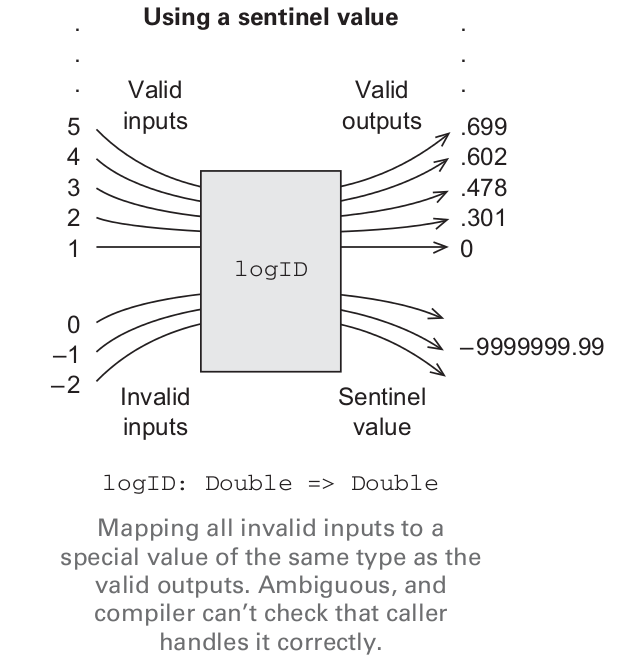
\includegraphics[scale=.15]{map-sentinel.png}
\end{center}
\end{frame}

\section{The Option data type}

\begin{frame}[fragile,t]
  \frametitle{Option 4 - The Option data type}
\begin{lstlisting}
sealed trait Option[+A]
case class Some[+A](get: A) extends Option[A]
case object None extends Option[Nothing]
\end{lstlisting}
\begin{center}
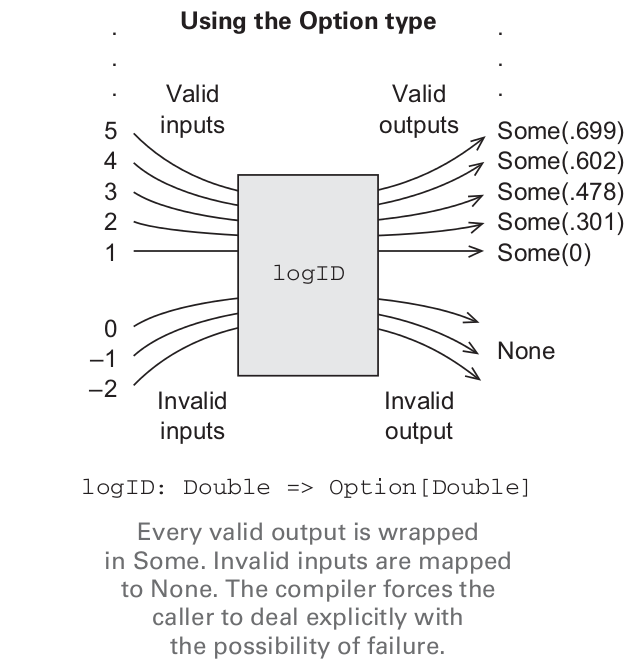
\includegraphics[scale=.15]{map-option.png}
\end{center}
\begin{lstlisting}
def mean(xs: Seq[Double]): Option[Double] =
  if (xs.isEmpty) None
  else Some(xs.sum / xs.length)
\end{lstlisting}
{\ttfamily mean} is now total
\end{frame}

\begin{frame}[fragile,t]
  \frametitle{{\ttfamily None} is not {\ttfamily null}!}
\begin{lstlisting}
sealed trait Option[+A]
case class Some[+A](get: A) extends Option[A]
case object None extends Option[Nothing]
\end{lstlisting}
  \begin{itemize}
    \item There is no such thing as a ``generic'' {\ttfamily None}
      \begin{itemize}
        \item {\ttfamily None} $\not\in$ {\ttfamily A}
        \item Can't return {\ttfamily None} from function that returns an {\ttfamily A}
      \end{itemize}
    \item Every usage of {\ttfamily None} must be assigned to a specific type
      \begin{itemize}
        \item {\ttfamily None:Option[A]} $\neq$ {\ttfamily None:Option[B]}, {\ttfamily None:Option[A]} $\not\in$ {\ttfamily Option[B]}
        %\item Just as {\ttfamily Nil:List[A]} $\neq$ {\ttfamily Nil:List[B]}, {\ttfamily Nil:List[A]} $\not\in$ {\ttfamily List[B]}
      \end{itemize}
    \item Type system prevents null pointer dereference
  \end{itemize}
\end{frame}

\begin{frame}[fragile,t]
  \frametitle{{\ttfamily Option} as a container}
\begin{lstlisting}
sealed trait Option[+A]
case class Some[+A](get: A) extends Option[A]
case object None extends Option[Nothing]
\end{lstlisting}
  Think of {\ttfamily Option[A]} as a {\ttfamily List[A]} with length $\le$ 1
  \begin{itemize}
    \item {\ttfamily None:Option[A]} $\approx$ {\ttfamily Nil:List[A]}
    \item {\ttfamily Some(a:A)} $\approx$ {\ttfamily List(a:A)}
  \end{itemize}
\end{frame}

\subsection{Usage patterns for Option - the Option functor}

\begin{frame}[fragile,t]
\frametitle{Usage patterns for Option}
\begin{lstlisting}
sealed trait Option[+A] {
  // Apply f if the Option is not None.
  def map[B](f: A => B): Option[B]

  // The B >: A says that the B type parameter must be
  // a supertype of A.
  def getOrElse[B>:A](default: => B): B

  // Apply f, which may fail, to the Option if not None.
  def flatMap[B](f: A => Option[B]): Option[B]

  // `ob: => Option[B]` means don't evaluate ob unless needed.
  // The argument is non-strict / evaulated lazily
  // (just like if-else short-circuiting) - see chapter 5!
  def orElse[B>:A](ob: => Option[B]): Option[B]

  // Convert Some to None if the value doesn't satisfy f.
  def filter(f: A => Boolean): Option[A]
}
case class Some[+A](get: A) extends Option[A]
case object None extends Option[Nothing]
\end{lstlisting}
\end{frame}

\begin{frame}[fragile,t]
\frametitle{Exercise 4.1}
\begin{lstlisting}
sealed trait Option[+A] {
  def map[B](f: A => B): Option[B] = this match {
    case None => None
    case Some(a) => Some(f(a))
  }

  def getOrElse[B>:A](default: => B): B = this match {
    case None => default
    case Some(a) => a
  }

  def flatMap[B](f: A => Option[B]): Option[B] =
    map(f) getOrElse None

  def orElse[B>:A](ob: => Option[B]): Option[B]
    map(Some(_)) getOrElse ob

  def filter(f: A => Boolean): Option[A] = {
    flatMap(a => if (f(a)) Some(a) else None)
  }
}
case class Some[+A](get: A) extends Option[A]
case object None extends Option[Nothing]
\end{lstlisting}
\end{frame}

\begin{frame}[fragile,t]
\frametitle{Usage scenarios for Option}
\begin{lstlisting}
sealed trait Option[+A] {
  def map[B](f: A => B): Option[B]
  def getOrElse[B>:A](default: => B): B
  def flatMap[B](f: A => Option[B]): Option[B]
  def orElse[B>:A](ob: => Option[B]): Option[B]
  def filter(f: A => Boolean): Option[A]
}
case class Some[+A](get: A) extends Option[A]
case object None extends Option[Nothing]
\end{lstlisting}
\begin{center}
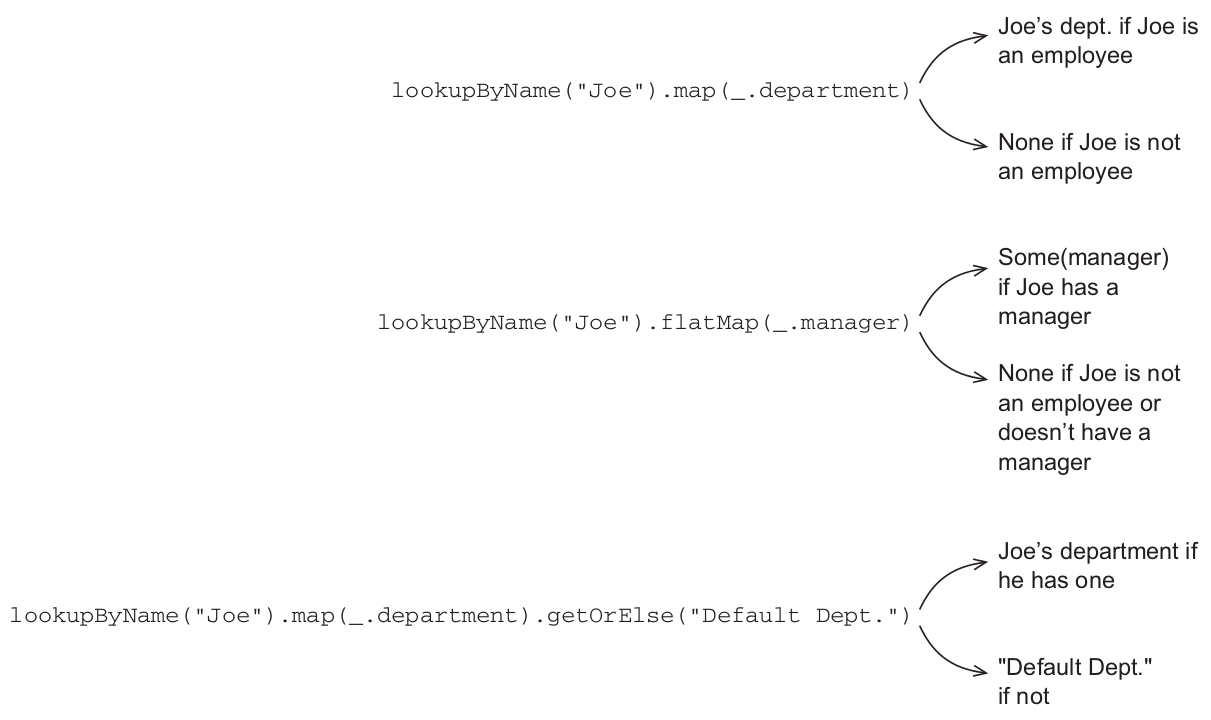
\includegraphics[scale=.15]{option-usage.png}
\end{center}
\end{frame}

\begin{frame}[fragile,t]
\frametitle{Usage patterns for Option}
\begin{lstlisting}
sealed trait Option[+A] {
  def map[B](f: A => B): Option[B]
  def getOrElse[B>:A](default: => B): B
  def flatMap[B](f: A => Option[B]): Option[B]
  def orElse[B>:A](ob: => Option[B]): Option[B]
  def filter(f: A => Boolean): Option[A]
}
case class Some[+A](get: A) extends Option[A]
case object None extends Option[Nothing]
\end{lstlisting}
\begin{enumerate}
  \item Some initial computation {\ttfamily f: A => Option[B]} may fail
  \item Apply further computations with {\ttfamily map}, {\ttfamily flatMap}
    \begin{itemize}
      %\item {\ttfamily map} when the subsequent computation is total
      %\item {\ttfamily flatMap} when the subsequent computation may itself fail
      \item Subsequent computations only run when there is still a value% to compute on
      %\item In error cases, subsequent computations are seamlessly bypassed, and {\ttfamily None} is carried through the computations
      \item In error cases, {\ttfamily None} is carried through the computations
    \end{itemize}
  \item Optionally {\ttfamily filter} on predicates to generate error
  \item Do error handling at end with {\ttfamily getOrElse} or {\ttfamily orElse}
    \begin{itemize}
      \item {\ttfamily getOrElse} provides default value
      \item {\ttfamily OrElse} provides new chain of computations to try
    \end{itemize}
\end{enumerate}
\end{frame}

\begin{frame}[fragile]
  \frametitle{Language Comparison}
  Scala:
\begin{lstlisting}
val dept: String =
  lookupByName("Joe").  // Impossible to forget None check.
  flatMap(_.dept).      // Type system does not allow you to.
  filter(_ != "Accounting").
  getOrElse("Default Dept")
\end{lstlisting}

  Python:
\begin{lstlisting}[language=Python]%
dept = "Default Dept"
employee = lookupByName("Joe")
# If you forget this line
if employee is not None:
  # this will raise AttributeError.
  department = employee.dept
  if (department is not None) and (department != "Accounting"):
    dept = department
\end{lstlisting}
\end{frame}

\begin{frame}[fragile,t]
  \frametitle{The Option functor}
\begin{lstlisting}
sealed trait Option[+A] {
  def map[B](f: A => B): Option[B]
  def flatMap[B](f: A => Option[B]): Option[B]
}
case class Some[+A](get: A) extends Option[A]
case object None extends Option[Nothing]
\end{lstlisting}
  \begin{center}
    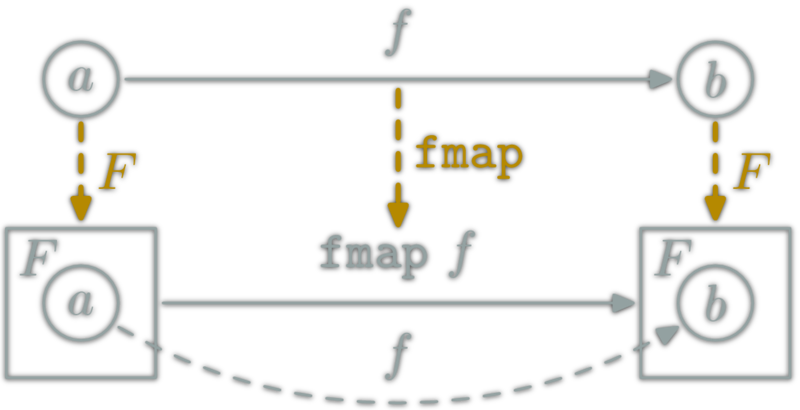
\includegraphics[scale=0.20]{boxfunctor.png}
  \end{center}
  \begin{enumerate}
    \item {\ttfamily map identity = identity}
    \item {\ttfamily map (f compose g) = (map f) compose (map g)}
  \end{enumerate}
  More in chapter 10!
\end{frame}

\subsection{Option composition and lifting - the monad laws}

\begin{frame}[fragile,t]
  \frametitle{Option composition - Exercise 4.3}
\begin{lstlisting}
sealed trait Option[+A] {
  def map[B](f: A => B): Option[B]
  def flatMap[B](f: A => Option[B]): Option[B]
}
case class Some[+A](get: A) extends Option[A]
case object None extends Option[Nothing]


// Return None if any input is None.
// Otherwise, apply the function to the values.
def map2[A,B,C](a:Option[A],b:Option[B])(f:(A,B)=>C):Option[C]
def flatMap2[A,B,C](a:Option[A],b:Option[B])(f:(A,B)=>Option[C]):Option[C]
def map3[A,B,C,D](a:Option[A],b:Option[B],c:Option[C])
                 (f:(A,B,C)=>D):Option[D]
\end{lstlisting}
\pause
\begin{lstlisting}
map2(a,b)(f) = a flatMap (aa => b map (bb => f(aa, bb)))
flatMap2(a,b)(f) = a flatMap (aa => b flatMap (bb => f(aa, bb)))
map3(a,b,c)(f) = a flatMap (aa => b flatMap(bb => c map (cc => f(aa, bb, cc))))
\end{lstlisting}
\end{frame}

\begin{frame}[fragile,t]
  \frametitle{Option lifting}
\begin{lstlisting}
sealed trait Option[+A] {
  def map[B](f: A => B): Option[B]
  def flatMap[B](f: A => Option[B]): Option[B]
}
case class Some[+A](get: A) extends Option[A]
case object None extends Option[Nothing]

def lift[A,B](f: A => B): Option[A] => Option[B] =
  _ map f
def flatLift[A,B](f: A => Option[B]): Option[A] => Option[B] =
  _ flatMap f
\end{lstlisting}
\begin{itemize}
  \item Take ordinary functions, and lift them to functions on {\ttfamily Option}
  \item Can design API of {\ttfamily A => B}, {\ttfamily A => Option[B]} functions
  \item Don't about writing all your functions to accept {\ttfamily Option[A]}
  \item Can lift buildin Java, Scala functions
\end{itemize}
\end{frame}

\begin{frame}[fragile,t]
  \frametitle{Option lifting}
\begin{lstlisting}
sealed trait Option[+A] {
  def map[B](f: A => B): Option[B]
  def flatMap[B](f: A => Option[B]): Option[B]
}
case class Some[+A](get: A) extends Option[A]
case object None extends Option[Nothing]

def lift[A,B](f: A => B): Option[A] => Option[B] =
  _ map f
def flatLift[A,B](f: A => Option[B]): Option[A] => Option[B] =
  _ flatMap f

val absO: Option[Double] => Option[Double] = lift(math.abs)
\end{lstlisting}
\begin{center}
  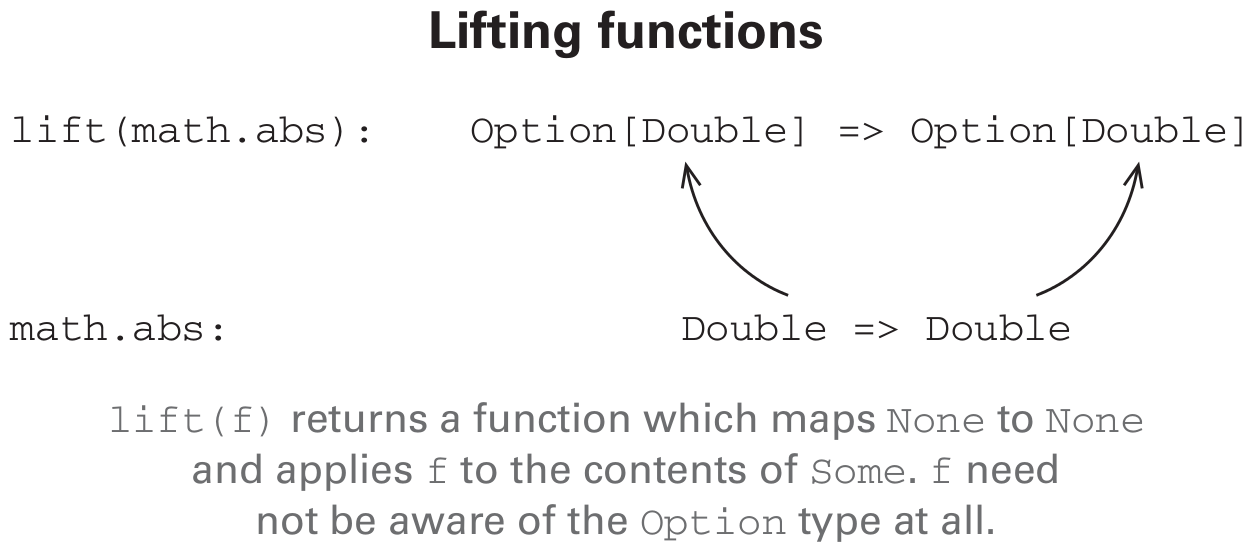
\includegraphics[scale=.13]{lift.png}
\end{center}
\end{frame}

\begin{frame}[fragile,t]
  \frametitle{Option monad}
\begin{lstlisting}
sealed trait Option[+A] {
  def map[B](f: A => B): Option[B]
  def flatMap[B](f: A => Option[B]): Option[B]
  val bind = flatMap
}
case class Some[+A](get: A) extends Option[A]
case object None extends Option[Nothing]

def unit[A](a: A): Option[A] =
  Some(a)
val return = unit
\end{lstlisting}
\begin{center}
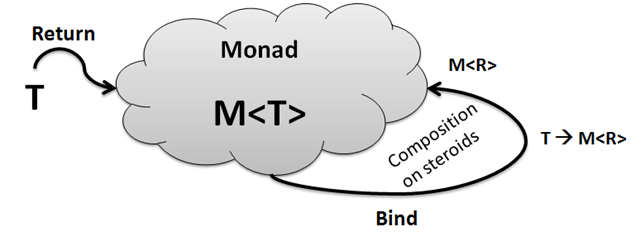
\includegraphics[scale=.35]{monad.png}
\end{center}
\end{frame}

\begin{frame}[fragile,t]
  \frametitle{Option monad}
\begin{lstlisting}
sealed trait Option[+A] {
  def map[B](f: A => B): Option[B]
  def flatMap[B](f: A => Option[B]): Option[B]
  val bind = flatMap
}
case class Some[+A](get: A) extends Option[A]
case object None extends Option[Nothing]

def unit[A](a: A): Option[A] =
  Some(a)
val return = unit
\end{lstlisting}
{\ttfamily unit(aa) bind f == f(aa)}

{\ttfamily a bind unit == a}

{\ttfamily a bind (aa=>f(aa) bind g) == (a bind f) bind g}
\end{frame}

\subsection{Wrapping exception-oriented APIs}

\begin{frame}[fragile]
  \frametitle{\subsecname}
\begin{lstlisting}
// We accept the A argument non-strictly,
// so we can catch any exceptions that
// occur while evaluating a and convert them to None.
def Try[A](a: => A): Option[A] =
  try Some(a)
  catch { case e: Exception => None }
\end{lstlisting}
\end{frame}

\section{The Either data type}

\section{Exercises}

\begin{frame}{\secname}
\end{frame}

\end{document}
